\section{Data}

The advent of mobile sensing techniques makes it possible to develop urban geography from social media source. Complement the infrequenly collect census. 
The wide use of social media brings the benefit of high disaggregate in terms of space and time, which supports to reach a wide range of individuals as well as sampling the rare movement, such as the night-time activity. 

Via Wechat, a wide used social media in China, 25481 individual volunteers were reached and returned feedbacks during the releasing time period (June - October, 2016). As Figure~\ref{fig:data_over} illustrates, each individual hands in his or her personal characteristics from social, economic and deomgraphic aspects. For privacy issue, all detailed personal information are desensitized to categorical levels. Finally, XX variables are created, falling into eight domains. Those domains give a generalized depiction of the individual characteristics and serve as the ingredients for the analysis of urban dynamics over diverse people. At the same time, individual is asked to tag the moving tracks according to his or her willingness. Individuals are motivated by a credit system which retains the track contribution and rewards who in the top contribution list. Over the time period of collection, XXX trips are collected and XX trips per individual. 


\begin{figure}[htb!]
 \centering % avoid the use of \begin{center}...\end{center} and use \centering instead (more compact)
 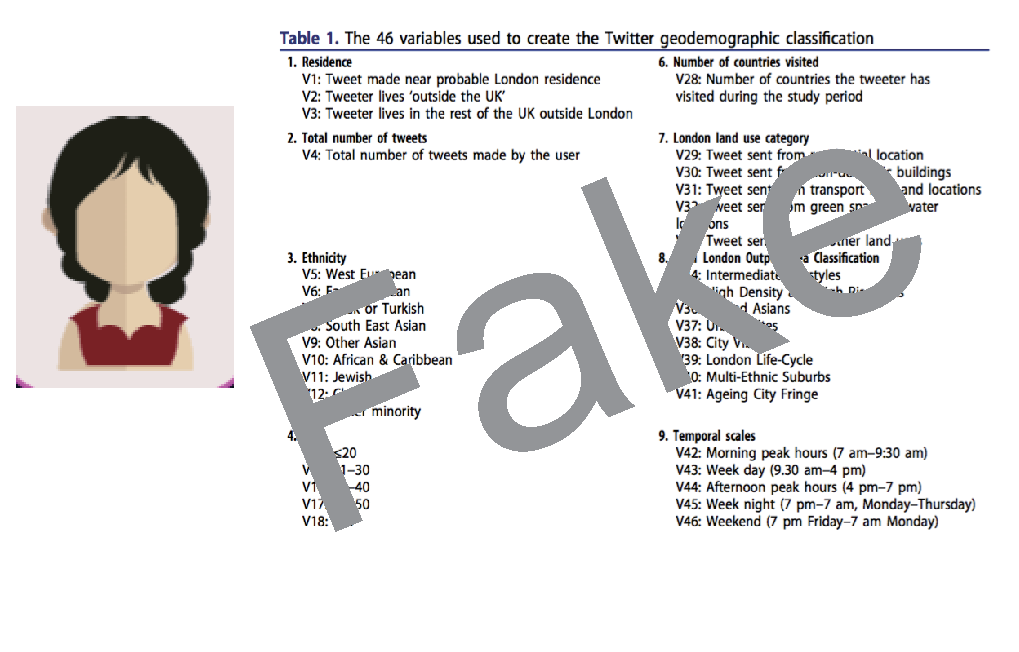
\includegraphics[width=\columnwidth]{pictures/data_over}
 \caption{Overview}
 \label{fig:data_over}
\end{figure}


Considering the caveat that self-selecting individuals are most unlikely to represent any clearly defined population~\cite{Longley2015}, a series of statistical analysis is performed to check whether it is rich enough to represent a wide range of human individuals in the city.

\textit{Overview} As Figure~\ref{fig:data_stat} shows, age... As reported in evenly sampled, geolocation is ...
\textit{Compared to Census} In the report (looking for some report), the penetration of mobile device is XXX, almost every XX people got a Mobile Phone in the urban. XX.  multiple social characteristics of a people is sampled, including income, education, etc. age and income distribution follows the social architecture. 



\begin{figure}[htb!]
 \centering % avoid the use of \begin{center}...\end{center} and use \centering instead (more compact)
 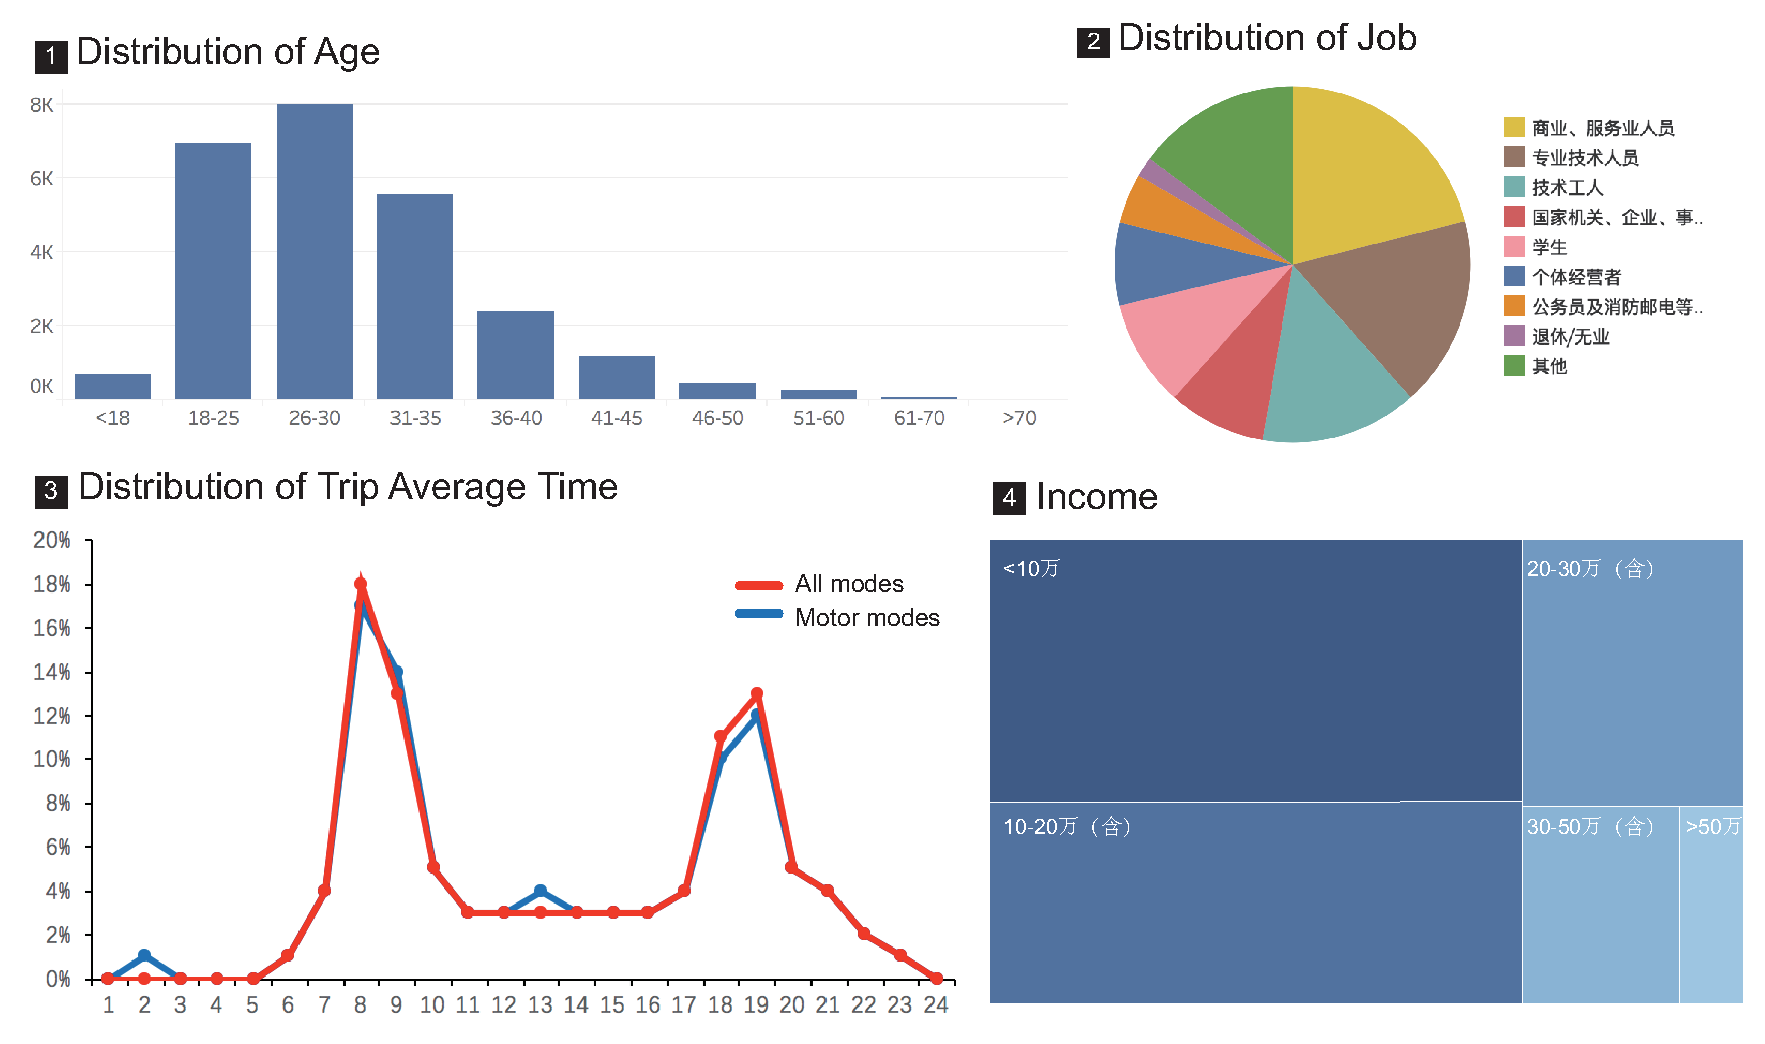
\includegraphics[width=\columnwidth]{pictures/data_detail}
 \caption{Statistical Overview of Social Characteristics}
 \label{fig:data_stat}
\end{figure}


